\chapter{Results}

\section{Term Statistics}

- display tf and maybe idf graph and table (one with stopwords and one without stopword)

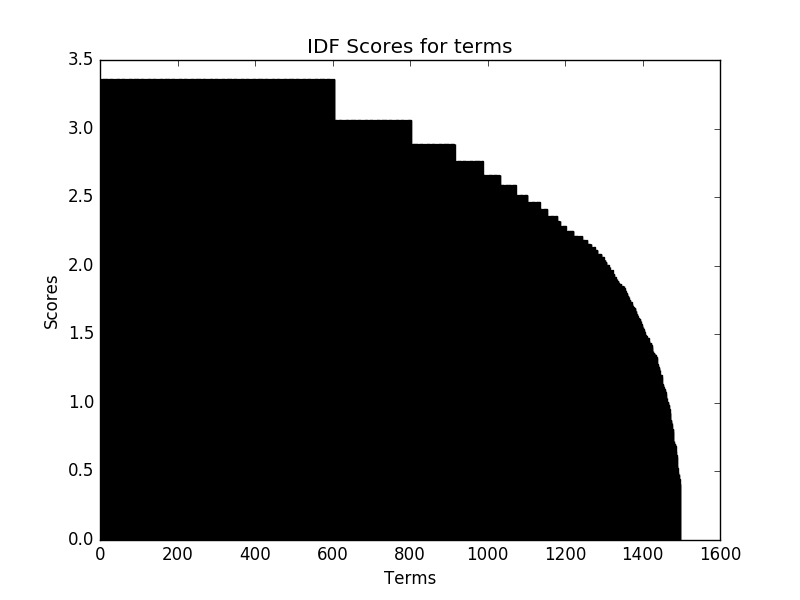
\includegraphics[width=0.95\textwidth]{images/graphs/idf}

- in total, there were `x` experts annotating images, however not all of these annotators were able to annotate the same number of images. The number of images annotated for each type of annoation methodology is displayed below


\section{Annotation Statistics}

\begin{table}[htb]
    \centering
    \begin{adjustbox}{center}
    \begin{tabular}{ | l | l | l | l | p{5cm} |}
    \hline
    & Text & Tags & Query & Relevance Assessment \\ \hline
    Count & 3172 & 1726 & 1626 & 191 \\ \hline
    Avg Time & 1 minute & 47 seconds & 12 seconds & 1 minute \\ \hline
    Total Time & 2 days, 23 hours & 19 hours, 46 minutes & 4 hours, 43 minutes & 5 hours, 4 minutes \\ \hline
    \end{tabular}
    \end{adjustbox}
    \caption{Annotation Statistics}
\end{table}

text
Textual annotation are the most time consuming annotation type to collect. Many images contain two or more highly relevant events or `important' objects. Describing these can take annotators up to several minutes each. This is opposed to all the other annotation methodologies where most images can be annotated in a minute or less.

tags
In terms of evaluation, tags may be the opposite of textual annotations; intuitively tags should be the best at training an image classifier and are expected to perform the worst when embedded a search task. Tags, however, may be very good at boosting the performance of other annotation types in the search task when combined. For instance, searching on the text \textit{and} tags fields may increase the scores of text annotation alone.

query
and therefore it is unknown how well the collected queries will perform in search or for training an image classifier. The level of detail in these annotations will be very low, since most queries should be short in length.
Much like tags, this annotation type will be very easy to collect. Formulating a query for an image should not takz a significant amount of time. There is the problem of bias \todo{Is there really? I should investigate this further}

\section{Retrieval Effectiveness}

- the results of each experiment are detailed below. first, each individual methodology, followed by each combination.\\
- tables of results go here\\
- outline the most effective combination here\\
- use of pre-trained model (Karpathy) for automatically captioning image had no impact on the retrieval performance.

\begin{table}[htb]
    \parbox{.45\linewidth}{
    \begin{tabular}{ | l | l | }
    \hline
    Metric & Score \\ \hline
	num\_q & 48 \\ \hline
	num\_ret & 476 \\ \hline
	num\_rel & 6708 \\ \hline
	num\_rel\_ret & 401 \\ \hline
	map & 0.3578 \\ \hline
	gm\_map & 0.1280 \\ \hline
	Rprec & 0.3635 \\ \hline
	bpref & 0.3627 \\ \hline
	recip\_rank & 0.9132 \\ \hline
	iprec\_at\_recall\_0.00 & 0.9433 \\ \hline
	iprec\_at\_recall\_0.10 & 0.6188 \\ \hline
	iprec\_at\_recall\_0.20 & 0.5354 \\ \hline
	iprec\_at\_recall\_0.30 & 0.4146 \\ \hline
	iprec\_at\_recall\_0.40 & 0.3104 \\ \hline
	iprec\_at\_recall\_0.50 & 0.3012 \\ \hline
	iprec\_at\_recall\_0.60 & 0.2896 \\ \hline
	iprec\_at\_recall\_0.70 & 0.2292 \\ \hline
	iprec\_at\_recall\_0.80 & 0.1875 \\ \hline
	iprec\_at\_recall\_0.90 & 0.1667 \\ \hline
	iprec\_at\_recall\_1.00 & 0.1667 \\ \hline
	P\_5 & 0.8833 \\ \hline
	P\_10 & 0.8354 \\ \hline
	P\_15 & 0.5569 \\ \hline
	P\_20 & 0.4177 \\ \hline
	P\_30 & 0.2785 \\ \hline
	P\_100 & 0.0835 \\ \hline
	P\_200 & 0.0418 \\ \hline
	P\_500 & 0.0167 \\ \hline
	P\_1000 & 0.0084 \\ \hline
    \end{tabular}
    \caption{Text}    
    }
    \hfill
    \parbox{.45\linewidth}{
    \begin{tabular}{ | l | l | }
    \hline
    Metric & Score \\ \hline
	num\_q & 32 \\ \hline
	num\_ret & 178 \\ \hline
	num\_rel & 5431 \\ \hline
	num\_rel\_ret & 12 \\ \hline
	map & 0.0008 \\ \hline
	gm\_map & 0.0000 \\ \hline
	Rprec & 0.0010 \\ \hline
	bpref & 0.0010 \\ \hline
	recip\_rank & 0.1234 \\ \hline
	iprec\_at\_recall\_0.00 & 0.1313 \\ \hline
	iprec\_at\_recall\_0.10 & 0.0000 \\ \hline
	iprec\_at\_recall\_0.20 & 0.0000 \\ \hline
	iprec\_at\_recall\_0.30 & 0.0000 \\ \hline
	iprec\_at\_recall\_0.40 & 0.0000 \\ \hline
	iprec\_at\_recall\_0.50 & 0.0000 \\ \hline
	iprec\_at\_recall\_0.60 & 0.0000 \\ \hline
	iprec\_at\_recall\_0.70 & 0.0000 \\ \hline
	iprec\_at\_recall\_0.80 & 0.0000 \\ \hline
	iprec\_at\_recall\_0.90 & 0.0000 \\ \hline
	iprec\_at\_recall\_1.00 & 0.0000 \\ \hline
	P\_5 & 0.0562 \\ \hline
	P\_10 & 0.0375 \\ \hline
	P\_15 & 0.0250 \\ \hline
	P\_20 & 0.0187 \\ \hline
	P\_30 & 0.0125 \\ \hline
	P\_100 & 0.0037 \\ \hline
	P\_200 & 0.0019 \\ \hline
	P\_500 & 0.0008 \\ \hline
	P\_1000 & 0.0004 \\ \hline
    \end{tabular}
    \caption{Tag}
    }
\end{table}

% query
% trec_eval results

\begin{table}[htb]
    \parbox{.45\linewidth}{
    \begin{tabular}{ | l | l | }
    \hline
    Metric & Score \\ \hline
	num\_q & 37 \\ \hline
	num\_ret & 343 \\ \hline
	num\_rel & 6297 \\ \hline
	num\_rel\_ret & 16 \\ \hline
	map & 0.0021 \\ \hline
	gm\_map & 0.0000 \\ \hline
	Rprec & 0.0038 \\ \hline
	bpref & 0.0037 \\ \hline
	recip\_rank & 0.1473 \\ \hline
	iprec\_at\_recall\_0.00 & 0.1473 \\ \hline
	iprec\_at\_recall\_0.10 & 0.0000 \\ \hline
	iprec\_at\_recall\_0.20 & 0.0000 \\ \hline
	iprec\_at\_recall\_0.30 & 0.0000 \\ \hline
	iprec\_at\_recall\_0.40 & 0.0000 \\ \hline
	iprec\_at\_recall\_0.50 & 0.0000 \\ \hline
	iprec\_at\_recall\_0.60 & 0.0000 \\ \hline
	iprec\_at\_recall\_0.70 & 0.0000 \\ \hline
	iprec\_at\_recall\_0.80 & 0.0000 \\ \hline
	iprec\_at\_recall\_0.90 & 0.0000 \\ \hline
	iprec\_at\_recall\_1.00 & 0.0000 \\ \hline
	P\_5 & 0.0649 \\ \hline
	P\_10 & 0.0432 \\ \hline
	P\_15 & 0.0288 \\ \hline
	P\_20 & 0.0216 \\ \hline
	P\_30 & 0.0144 \\ \hline
	P\_100 & 0.0043 \\ \hline
	P\_200 & 0.0022 \\ \hline
	P\_500 & 0.0009 \\ \hline
	P\_1000 & 0.0004 \\ \hline
    \end{tabular}
    \caption{Query}
    }
    \parbox{.45\linewidth}{
    \begin{tabular}{ | l | l | }
    \hline
    Metric & Score \\ \hline

    \end{tabular}
    \caption{Relevance Assessment}
    }
\end{table}

